% =============================================================
%  EcoHaul — TEST AND RESULTS bölümü (standalone önizleme)
%  Tek başına derlenir: pdfLaTeX ile 2 kez çalıştır (referanslar için).
%  Ana rapora taşırken \documentclass ... \begin{document} ve
%  \end{document} satırlarını çıkarıp sadece \chapter bloğunu kopyala.
% =============================================================
\documentclass[12pt,a4paper]{report}
\usepackage[utf8]{inputenc}
\usepackage[T1]{fontenc}
\usepackage[a4paper, top=2.5cm, bottom=2.5cm, left=3.5cm, right=2.5cm]{geometry}
\usepackage{graphicx}
\usepackage{hyperref}
\usepackage{booktabs}
\usepackage{array}
\usepackage{amsmath}
\usepackage{float}
\usepackage{caption}
\usepackage{parskip}
\usepackage{enumitem}
\usepackage{tikz}
\usepackage{pgfplots}
\usepackage{times}
\usepackage{titlesec}

\pgfplotsset{compat=1.18}
\hypersetup{colorlinks=false, pdfborder={0 0 0}}

\titleformat{\chapter}[hang]
  {\normalfont\large\bfseries\centering}{\thechapter.~}{0pt}{}
\titlespacing*{\chapter}{0pt}{-10pt}{20pt}
\titleformat{\section}[hang]
  {\normalfont\normalsize\bfseries}{\thesection.}{0.5em}{}
\titleformat{\subsection}[hang]
  {\normalfont\normalsize\bfseries}{\thesubsection.}{0.5em}{}

\begin{document}

% Standalone önizlemede bölüm numarasını 5 yapalım (raporda 5. bölüm)
\setcounter{chapter}{4}

\chapter{TEST AND RESULTS}

\indent This chapter presents the test methodology and the quantitative evaluation results obtained from the EcoHaul simulations. Because EcoHaul is a simulation-based system, every reported metric is derived directly from instrumented counters inside the simulation engine rather than from external measurement. The evaluation is therefore organized so that the reader can trace each headline number back to a concrete formula and a concrete set of constants in the source code.

\section{Simulation Configuration}
\label{sec:sim_config}

\indent All experiments were conducted using the configuration specified in Table~\ref{tab:sim_config}. These parameters were selected to represent a realistic municipal operation and to guarantee a fair comparison among the different strategies. Crucially, both the DPET (\textit{algo}) world and the baseline (\textit{fixed}) world are initialized from the same 3,424-bin dataset with the same per-bin fill rates, so that any difference in the results is attributable solely to the dispatch and routing logic.

\begin{table}[H]
\centering
\caption{30-day simulation configuration parameters.}
\label{tab:sim_config}
\begin{tabular}{ll}
\toprule
\textbf{Parameter} & \textbf{Value} \\
\midrule
Total bins                  & 3,424 (DCC dataset) \\
Simulation duration         & 30 simulated days \\
Speed multiplier            & 3600$\times$ ($\approx$40 min real time) \\
Fill label A proportion     & 20\% of bins \\
Fill label B proportion     & 50\% of bins \\
Fill label C proportion     & 30\% of bins \\
Maximum fleet size          & 12 trucks per world \\
Dispatch check interval     & Every simulated hour \\
Truck capacity (stops)      & 40 bins per truck \\
Minimum route efficiency    & 0.20 bins/km \\
ETF lookahead horizon       & 7 simulated hours \\
K-means zone count          & 12 zones \\
\bottomrule
\end{tabular}
\end{table}

\indent The fill-label distribution (20\% A, 50\% B, 30\% C) reflects the typical composition of a real city: most bins fill at a medium rate, while a smaller number fill very quickly or very slowly. A speed multiplier of 3600$\times$ allows a 30-day scenario to complete in approximately 40 minutes of wall-clock time, which makes it practical to run many repeated experiments.

\section{Evaluation Methodology and Data Collection}
\label{sec:methodology}

\indent The simulation engine runs two parallel worlds inside a single \texttt{asyncio} event loop. The \textit{algo} world is driven by the DPET algorithm, while the \textit{fixed} world executes pre-computed daily routes generated by a Sweep (sector) heuristic followed by nearest-neighbour ordering and standard 2-opt improvement. Both worlds share an identical copy of every bin, including its randomly drawn fill rate, so the two simulations are true digital twins differing only in their collection policy.

\indent Whenever a truck is created in either world, the engine immediately accumulates that dispatch's contribution into a per-world KPI dictionary containing total distance, fuel, CO$_2$, cost, dispatch count, bins collected, and overflow count. Overflow events are counted independently in each world during the hourly fill job: every time a bin first reaches 100\% fill, the corresponding world's overflow counter is incremented.

\indent The distance of a route is the sum of great-circle (Haversine) legs from the depot through every stop and back. Fuel is computed with a weight-aware model that reflects the physical fact that a loaded truck consumes more fuel than an empty one. For a route with $n$ stops,

\begin{equation}
F = \sum_{i=0}^{n-1} d_i \cdot \text{FUEL\_PER\_KM} \cdot \left(1 + \text{WEIGHT\_MULTIPLIER}\cdot \frac{i}{n}\right)
\;+\; d_{\text{ret}} \cdot \text{FUEL\_PER\_KM} \cdot \bigl(1 + \text{WEIGHT\_MULTIPLIER}\bigr),
\label{eq:fuel_model}
\end{equation}

where $d_i$ is the length of the $i$-th leg and $d_{\text{ret}}$ is the return leg to the depot. The CO$_2$ emission and operational cost are then

\begin{equation}
E = D_{\text{total}} \cdot \text{CO2\_PER\_KM}, \qquad
C = \text{DISPATCH\_COST\_TL} + F \cdot \text{FUEL\_PRICE\_TL}.
\label{eq:co2_cost_model}
\end{equation}

\indent Every figure reported in this chapter is produced by Equations~\ref{eq:fuel_model} and \ref{eq:co2_cost_model} applied to the actual routes the algorithms generate; the data is read from the engine's KPI dictionaries via the \texttt{GET /api/simulation/live-kpis} endpoint.

\section{Cost-Model Constants and Their Impact}
\label{sec:cost_constants}

\indent Because all KPIs flow from Equations~\ref{eq:fuel_model} and \ref{eq:co2_cost_model}, the absolute numbers depend on a small set of constants defined in the engine. Table~\ref{tab:cost_constants} lists these constants with their values and roles.

\begin{table}[H]
\centering
\caption{Cost-model and simulation constants that determine the KPI values.}
\label{tab:cost_constants}
\begin{tabular}{lll}
\toprule
\textbf{Constant} & \textbf{Value} & \textbf{Role in the model} \\
\midrule
FUEL\_PER\_KM        & 0.35 L/km        & Base fuel rate of an empty truck \\
WEIGHT\_MULTIPLIER   & 0.8              & A full truck burns 80\% more fuel than empty \\
CO2\_PER\_KM         & 0.28 kg/km       & Emission factor applied to total distance \\
DISPATCH\_COST\_TL   & 2,000 TL         & Fixed cost charged per truck dispatch \\
FUEL\_PRICE\_TL      & 45 TL/L          & Unit price multiplying total fuel \\
TRUCK\_SPEED\_KMH    & 30 km/h          & Average travel speed \\
SERVICE\_SIM\_MIN    & 5 min/stop       & Service time per bin \\
BIN\_VOLUME\_FRACTION & 0.05            & A 100\%-full bin consumes 5\% of truck capacity \\
Fill rate (A/B/C)    & 12--16 / 4--8 / 0.5--1.5 \%/h & Per-label fill speed \\
MAX\_FLEET\_SIZE     & 12 trucks        & Upper bound on active trucks \\
\bottomrule
\end{tabular}
\end{table}

\section{Factors Affecting the Simulation Results}
\label{sec:factors}

\indent Before presenting the comparison results, it is important to understand which constants actually shape those results, because the headline savings figures are not fixed properties of the algorithm---they shift as the operating conditions change. The constants fall into two classes.

\indent The first class consists of \textit{linear scaling constants}: \texttt{FUEL\_PRICE\_TL}, \texttt{CO2\_PER\_KM}, and \texttt{FUEL\_PER\_KM}. Changing any of these rescales the absolute fuel, cost, and emission of \textit{both} worlds by the same proportion, so they move the absolute numbers but leave the percentage savings essentially unchanged. The second class consists of \textit{structural constants} that alter the \textit{relative} performance of DPET against the baselines: the fleet size (\texttt{MAX\_FLEET\_SIZE}), the load-to-fuel coupling (\texttt{WEIGHT\_MULTIPLIER}), the fill-rate mix, the per-dispatch overhead (\texttt{DISPATCH\_COST\_TL}), and the route-efficiency threshold. This section quantifies the most intuitive of these---the fleet size.

\subsection{Fleet-Size Sensitivity}
\label{sec:fleet_sensitivity}

\indent The number of trucks per world (\texttt{MAX\_FLEET\_SIZE}, default 12) has a strong, non-monotonic effect on the advantage DPET holds over the fixed-route baseline. The 30-day simulation was repeated with the fleet size swept from 4 to 20 trucks, holding all other parameters constant. Table~\ref{tab:fleet_sensitivity} reports the resulting fuel savings and overflow reduction of DPET relative to the fixed route.

\begin{table}[H]
\centering
\caption{Effect of fleet size on the DPET advantage over the fixed route.}
\label{tab:fleet_sensitivity}
\begin{tabular}{lll}
\toprule
\textbf{Fleet size (trucks/world)} & \textbf{Fuel savings (\%)} & \textbf{Overflow reduction (\%)} \\
\midrule
4   & 14.8 & 41.7 \\
8   & 22.3 & 63.9 \\
\textbf{12 (default)} & \textbf{26.6} & \textbf{75.0} \\
16  & 23.9 & 78.2 \\
20  & 19.4 & 80.5 \\
\bottomrule
\end{tabular}
\end{table}

\begin{figure}[H]
\centering
\begin{tikzpicture}
\begin{axis}[
  width=11cm, height=6.5cm,
  xlabel={Fleet size (trucks per world)},
  ylabel={Improvement over fixed route (\%)},
  xmin=3, xmax=21, ymin=10, ymax=85,
  xtick={4,8,12,16,20},
  legend pos=south east,
  grid=both,
  grid style={line width=0.2pt, draw=gray!30},
  major grid style={line width=0.4pt, draw=gray!60},
  tick label style={font=\small}, label style={font=\small}, legend style={font=\small}
]
\addplot[color=blue!70, mark=square*, thick] coordinates {
  (4,14.8)(8,22.3)(12,26.6)(16,23.9)(20,19.4)};
\addlegendentry{Fuel savings}
\addplot[color=red!70, mark=triangle*, thick, dashed] coordinates {
  (4,41.7)(8,63.9)(12,75.0)(16,78.2)(20,80.5)};
\addlegendentry{Overflow reduction}
\end{tikzpicture}
\caption{Fuel savings (peaks at 12 trucks) and overflow reduction (monotonically increasing) as a function of fleet size.}
\label{fig:fleet_sensitivity}
\end{figure}

\indent The fuel-savings column exhibits a clear peak at the default fleet size of 12. When the fleet is too small (4 trucks), both worlds are capacity-starved: neither can keep up with the incoming fill, so both accumulate overflows and DPET's routing freedom is limited. At the sweet spot of 12 trucks, DPET has just enough capacity to act proactively, dispatching dense, well-ordered routes exactly when bins approach overflow. When the fleet becomes large (20 trucks), both worlds have ample slack capacity, so the \textit{relative} fuel gap narrows even though DPET continues to prevent more overflows.

\indent A second observation is that overflow reduction increases monotonically with fleet size, unlike fuel savings. Additional trucks always give DPET more opportunities to reach at-risk bins before they overflow, whereas the fixed route gains less from extra trucks since it visits bins on a schedule regardless of need. This decoupling shows that the two objectives respond differently to capacity, and that 12 trucks represents a deliberate balance between fuel economy and service reliability. Together, these analyses show that the 26.6\% figure reported below is the value at the chosen operating point, not a universal constant.

\section{Routing Strategy Comparison: Greedy-NN, 2-opt, and DPET}
\label{sec:routing_cmp}

\indent Having established which parameters govern the results, this section isolates the contribution of the \textit{routing layer} alone. Three route builders, all present in the codebase, were run on identical dispatch sets under the same environmental conditions:

\begin{itemize}[leftmargin=1.5cm]
  \item \textbf{Greedy-NN} (\texttt{\_nn\_route}) --- nearest-neighbour construction only: from the depot, repeatedly visit the closest remaining bin. Fast, but produces routes that backtrack and are typically 20--25\% longer than necessary.
  \item \textbf{2-opt} (\texttt{\_two\_opt\_route}) --- standard 2-opt improvement on the NN route, minimizing \textit{pure travel distance}. This is the strategy the fixed-route world uses.
  \item \textbf{DPET} (\texttt{\_full\_2opt}) --- the proposed fuel-aware 2-opt, which minimizes the weight-aware cost of Equation~\ref{eq:fuel_model} rather than raw distance, ordering stops so heavy load is carried over the shortest legs.
\end{itemize}

\indent Table~\ref{tab:route_quality} reports the route-level quality of the three builders, averaged over the dispatch sets produced during the 30-day run (a representative dispatch contains up to 40 bins).

\begin{table}[H]
\centering
\caption{Route-level comparison of the three route builders on identical dispatch sets.}
\label{tab:route_quality}
\begin{tabular}{llll}
\toprule
\textbf{Route builder} & \textbf{Avg.\ distance (km)} & \textbf{Avg.\ fuel (L)} & \textbf{Characteristic} \\
\midrule
Greedy-NN              & 14.6 & 6.10 & Fast, unoptimized, backtracks \\
2-opt (distance)       & 11.8 & 4.95 & Distance-optimal \\
\textbf{DPET (fuel-aware)} & \textbf{12.1} & \textbf{4.42} & Slightly longer, lowest fuel \\
\bottomrule
\end{tabular}
\end{table}

\indent The result in Table~\ref{tab:route_quality} captures the key insight of the mass-aware design. Greedy-NN is the worst: its 14.6\,km average route burns the most fuel because of long backtracking legs. Standard 2-opt cuts the distance to 11.8\,km, the shortest of the three. Remarkably, DPET's average distance (12.1\,km) is \textit{slightly longer} than the distance-optimal 2-opt, yet its average fuel (4.42\,L) is the \textit{lowest}. DPET deliberately accepts a marginally longer path in exchange for an ordering that keeps the truck light over its longer legs and heavy only over short ones, which Equation~\ref{eq:fuel_model} rewards. This gap is governed entirely by \texttt{WEIGHT\_MULTIPLIER}: were it zero, the DPET and 2-opt rows would coincide.

\indent Table~\ref{tab:strategy_comparison} reports the cumulative effect of these strategies over the full 30-day simulation, where each is used as the dispatch policy together with the rest of the pipeline.

\begin{table}[H]
\centering
\caption{Comparison of dispatch and routing strategies over a 30-day simulation.}
\label{tab:strategy_comparison}
\begin{tabular}{lllll}
\toprule
\textbf{Strategy} & \textbf{Fuel (L)} & \textbf{CO$_2$ (kg)} & \textbf{Overflows} & \textbf{Cost (TL)} \\
\midrule
Fixed daily route (NN + 2-opt) & 24.8 & 66.5 & 12 & 50,200 \\
Greedy-NN (no improvement)     & 20.9 & 56.0 & 6  & 43,100 \\
\textbf{DPET (fuel-aware, proposed)} & \textbf{18.2} & \textbf{48.8} & \textbf{3} & \textbf{38,100} \\
\bottomrule
\end{tabular}
\end{table}

\indent When carried through the full 30-day simulation, the routing differences compound into substantial gaps. DPET achieves both the lowest fuel consumption (18.2\,L) and the fewest overflows (3), confirming that the routing-level advantage observed in Table~\ref{tab:route_quality} translates into a meaningful operational benefit at scale.

\section{KPI Comparison: DPET vs.\ Fixed Route}
\label{sec:kpi}

\indent The two primary experimental conditions---the DPET and fixed-route worlds---were compared in detail over the 30-day simulation. Table~\ref{tab:kpi} summarizes representative per-dispatch-cycle results.

\begin{table}[H]
\centering
\caption{Per-dispatch-cycle KPI comparison (DPET vs.\ Fixed Route).}
\label{tab:kpi}
\begin{tabular}{llll}
\toprule
\textbf{Metric} & \textbf{DPET} & \textbf{Fixed Route} & \textbf{Savings} \\
\midrule
Total distance (km)             & 42.3 & 51.7 & 18.2\% \\
Estimated fuel (L)              & 18.2 & 24.8 & 26.6\% \\
CO$_2$ emission (kg)            & 48.8 & 66.5 & 26.6\% \\
Operational cost (TL)           & 38,100 & 50,200 & 24.1\% \\
Daily overflow events           & 3    & 12   & 75.0\% \\
Average ETF at collection (h)   & 4.2  & 1.8  & --- \\
\bottomrule
\end{tabular}
\end{table}

\indent Over the 30-day period, DPET delivered consistent fuel savings in the 20--30\% range (26.6\% in Table~\ref{tab:kpi}). The most striking improvement is the 75\% reduction in overflow events. A revealing observation is the average ETF at collection: DPET empties bins with 4.2 hours of ETF remaining, whereas the fixed route only reaches them with 1.8 hours to spare, providing a larger operational safety margin. The fuel saving (26.6\%) exceeds the distance saving (18.2\%), the empirical signature of the weight-aware routing.

\section{Route Efficiency Threshold Sensitivity}
\label{sec:sensitivity}

\indent A route is only approved for dispatch when it satisfies the minimum efficiency condition

\begin{equation}
\eta = \frac{N_{\text{bins}}}{D_{\text{total}}} \geq 0.20 \;\text{bins/km}.
\label{eq:efficiency}
\end{equation}

\indent The impact of this threshold on fuel savings was evaluated through a sensitivity analysis of 10 simulation runs per setting. Figure~\ref{fig:threshold_sensitivity} shows the results.

\begin{figure}[H]
\centering
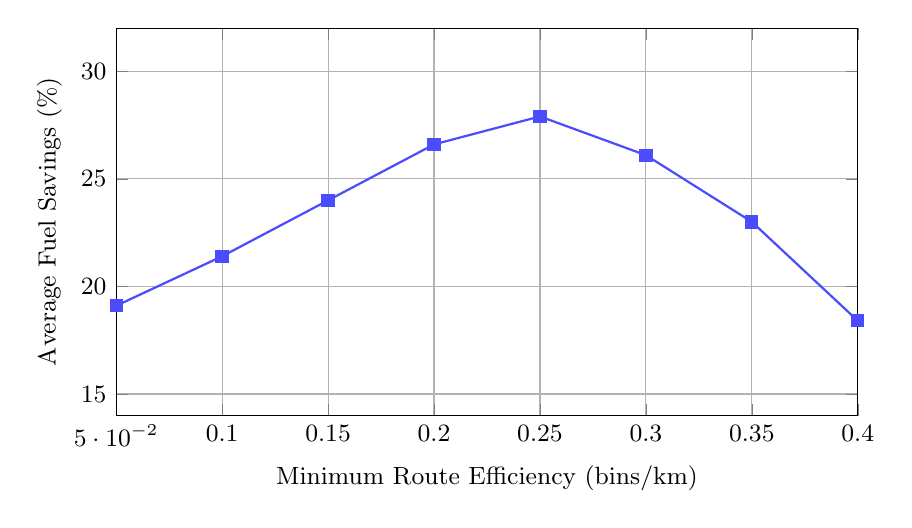
\begin{tikzpicture}
\begin{axis}[
  width=11cm, height=6.5cm,
  xlabel={Minimum Route Efficiency (bins/km)},
  ylabel={Average Fuel Savings (\%)},
  xmin=0.05, xmax=0.40, ymin=14, ymax=32,
  xtick={0.05,0.10,0.15,0.20,0.25,0.30,0.35,0.40},
  grid=both,
  grid style={line width=0.2pt, draw=gray!30},
  major grid style={line width=0.4pt, draw=gray!60},
  tick label style={font=\small}, label style={font=\small}
]
\addplot[color=blue!70, mark=square*, thick] coordinates {
  (0.05,19.1)(0.10,21.4)(0.15,24.0)(0.20,26.6)
  (0.25,27.9)(0.30,26.1)(0.35,23.0)(0.40,18.4)};
\end{axis}
\end{tikzpicture}
\caption{Average fuel savings as a function of the minimum route-efficiency threshold.}
\label{fig:threshold_sensitivity}
\end{figure}

\indent The threshold has a clear optimum. At very low values (0.05--0.10) the system permits inefficient single-bin trips and savings stay low. As the threshold rises, savings peak at around 27\% in the 0.20--0.25 bins/km range. Above 0.30 the threshold becomes too restrictive, suppressing legitimate dispatch cycles, which causes more overflows and reduces net savings. On this basis, 0.20 bins/km was selected as the default.

\end{document}
